\documentclass{source/Paper}

\major{信息工程}
\name{姓名}
\articletitle{喇叭天线的幅射特性测量及CST仿真}
\stuid{3000000}
\college{信息与电子工程学院}
\date{\today}
\course{电磁场与电磁波}
\instructor{指导老师}
\Abstract{大不自多,海纳江河。惟学无际,际于天地。形上谓道兮,形下谓器。礼主别异兮,乐主和同。知其不二兮,尔听斯聪!国有成均,在浙之滨。昔言求是,实启尔求真。习坎示教,始见经纶。无曰已是,无曰遂真。靡革匪因,靡故匪新。何以新之?开物前民。嗟尔髦士,尚其有闻。念哉典学,思睿观通。有文有质,有农有工。兼总条贯,知至知终。成章乃达,若金之在熔。尚亨于野,无吝于宗。树我邦国,天下来同。}
\Keyword{大不自多;大不自多}

\begin{document}
    \makeheader
    \section{第一}
        \subsection{第一}
            大不自多,海纳江河。惟学无际,际于天地。形上谓道兮,形下谓器。礼主别异兮,乐主和同。知其不二兮,尔听斯聪!国有成均,在浙之滨。昔言求是,实启尔求真。习坎示教,始见经纶。无曰已是,无曰遂真。靡革匪因,靡故匪新。何以新之?开物前民。嗟尔髦士,尚其有闻。念哉典学,思睿观通。有文有质,有农有工。兼总条贯,知至知终。成章乃达,若金之在熔。尚亨于野,无吝于宗。树我邦国,天下来同。

            \lstinputlisting[
                language = Verilog,
                title = {代码块测试(直接从文件导入)}
            ]{code/code_test.v}

            \begin{lstlisting}[language = Verilog, title = {代码块测试(直接插入)}]
module dffre (
    d, en, r, clk, q
);
    parameter n = 1;
    input en,r,clk;
    input [n-1:0] d;
    output [n-1:0] q;
    reg [n-1:0] q;
    always @(posedge clk) begin
        if(r) q = {n{1'b0}};
        else if(en) q = d;
            else q = q;
    end
endmodule
            \end{lstlisting}

            \begin{figure}[H]
                \centering
                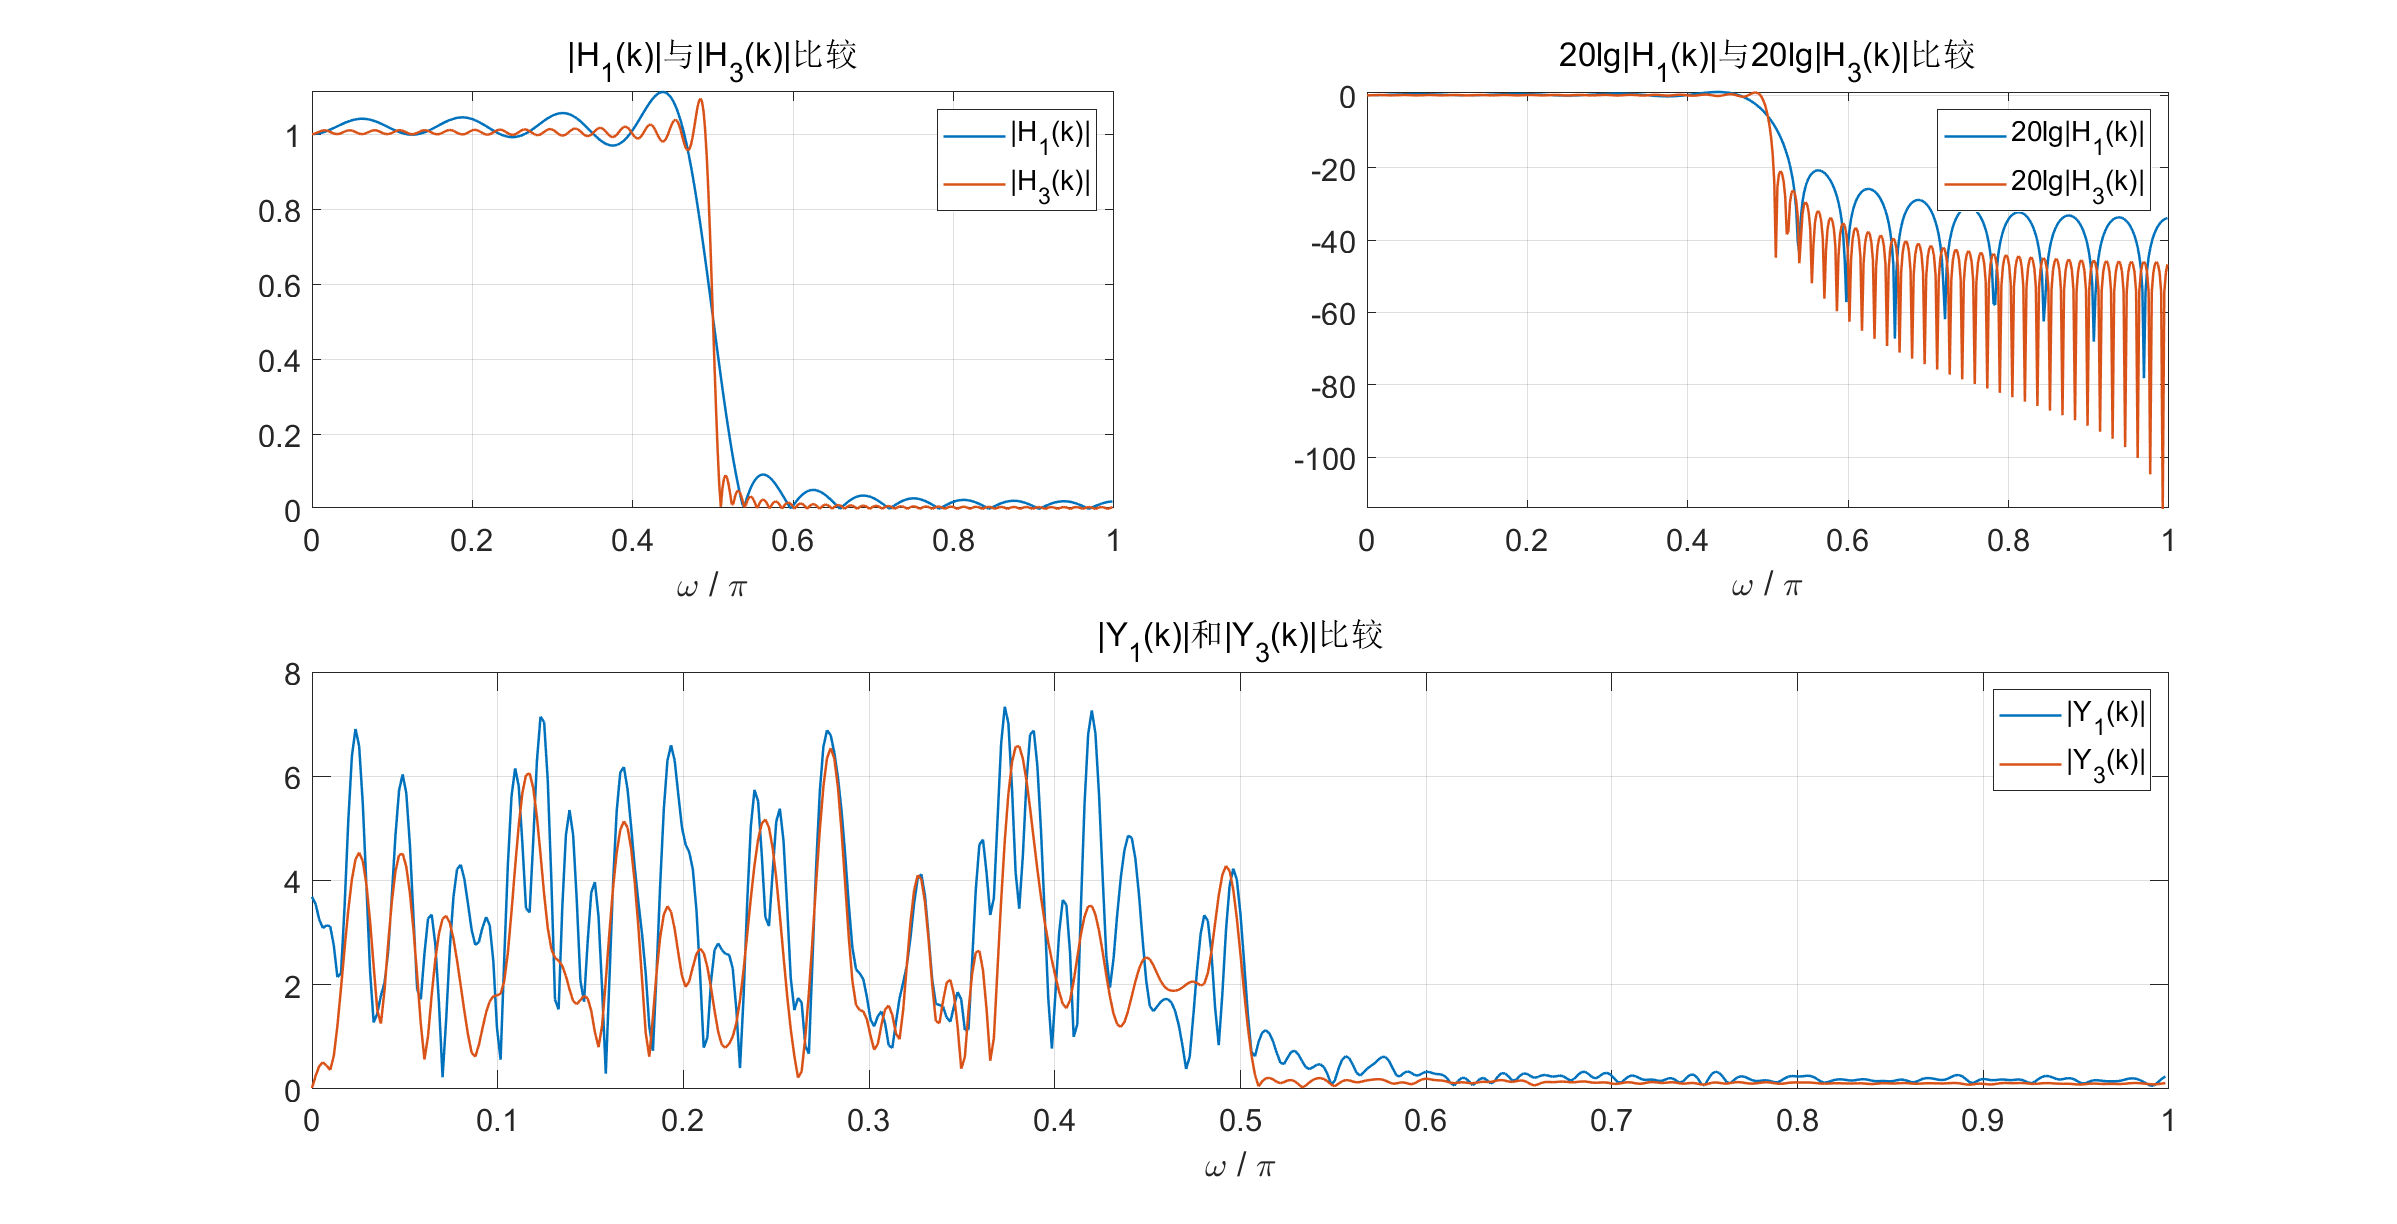
\includegraphics[width = 1\textwidth]{pic1}
                \caption{图片测试}
            \end{figure}


    \section{第二}
            \subsection{第一}
            大不自多,海纳江河。惟学无际,际于天地。形上谓道兮,形下谓器。礼主别异兮,乐主和同。知其不二兮,尔听斯聪!国有成均,在浙之滨。昔言求是,实启尔求真。习坎示教,始见经纶。无曰已是,无曰遂真。靡革匪因,靡故匪新。何以新之?开物前民。嗟尔髦士,尚其有闻。念哉典学,思睿观通。有文有质,有农有工。兼总条贯,知至知终。成章乃达,若金之在熔。尚亨于野,无吝于宗。\Footnote{脚注测试}树我邦国,天下来同。
            \begin{table}[H]
                \centering
                \caption{表格测试}
                \begin{tabular}{|c|c|c|c|c|c|c|c|c|}
                \hline
                state                 & ld & st & addr{[}31:11{]} == tag & valid & dirty & l2\_ack & write\_done & nextstate                   \\ \hline
                \multirow{4}{*}{Idle} & 0  & 0  & -                      & -     & -     & -       & -           & Idle                        \\ \cline{2-9} 
                                    & 0  & 1  & -                      & -     &       & -       & -           & \multirow{3}{*}{CompareTag} \\ \cline{2-8}
                                    & 1  & 0  & -                      & -     &       & -       & -           &                             \\ \cline{2-8}
                                    & 1  & 1  & -                      & -     &       & -       & -           &                             \\ \hline
            \end{tabular}
            \end{table}
\end{document}